\documentclass[tikz,border=8pt]{standalone}

\usepackage{xcolor}
\usetikzlibrary{calc}

% ---- 11 种高饱和、鲜亮配色 ----
\definecolor{barA}{HTML}{1A6FDF} % 亮蓝
\definecolor{barB}{HTML}{27C93F} % 鲜绿
\definecolor{barC}{HTML}{FF3B30} % 醒目红
\definecolor{barD}{HTML}{8E44FF} % 电光紫
\definecolor{barE}{HTML}{FF9500} % 明橙
\definecolor{barF}{HTML}{00C2D1} % 亮青
\definecolor{barG}{HTML}{E5177B} % 玫红
\definecolor{barH}{HTML}{FFD500} % 亮黄
\definecolor{barI}{HTML}{00A878} % 翡翠绿
\definecolor{barJ}{HTML}{7B4DFF} % 靛紫
\definecolor{barK}{HTML}{FF6B00} % 焦橙

\begin{document}

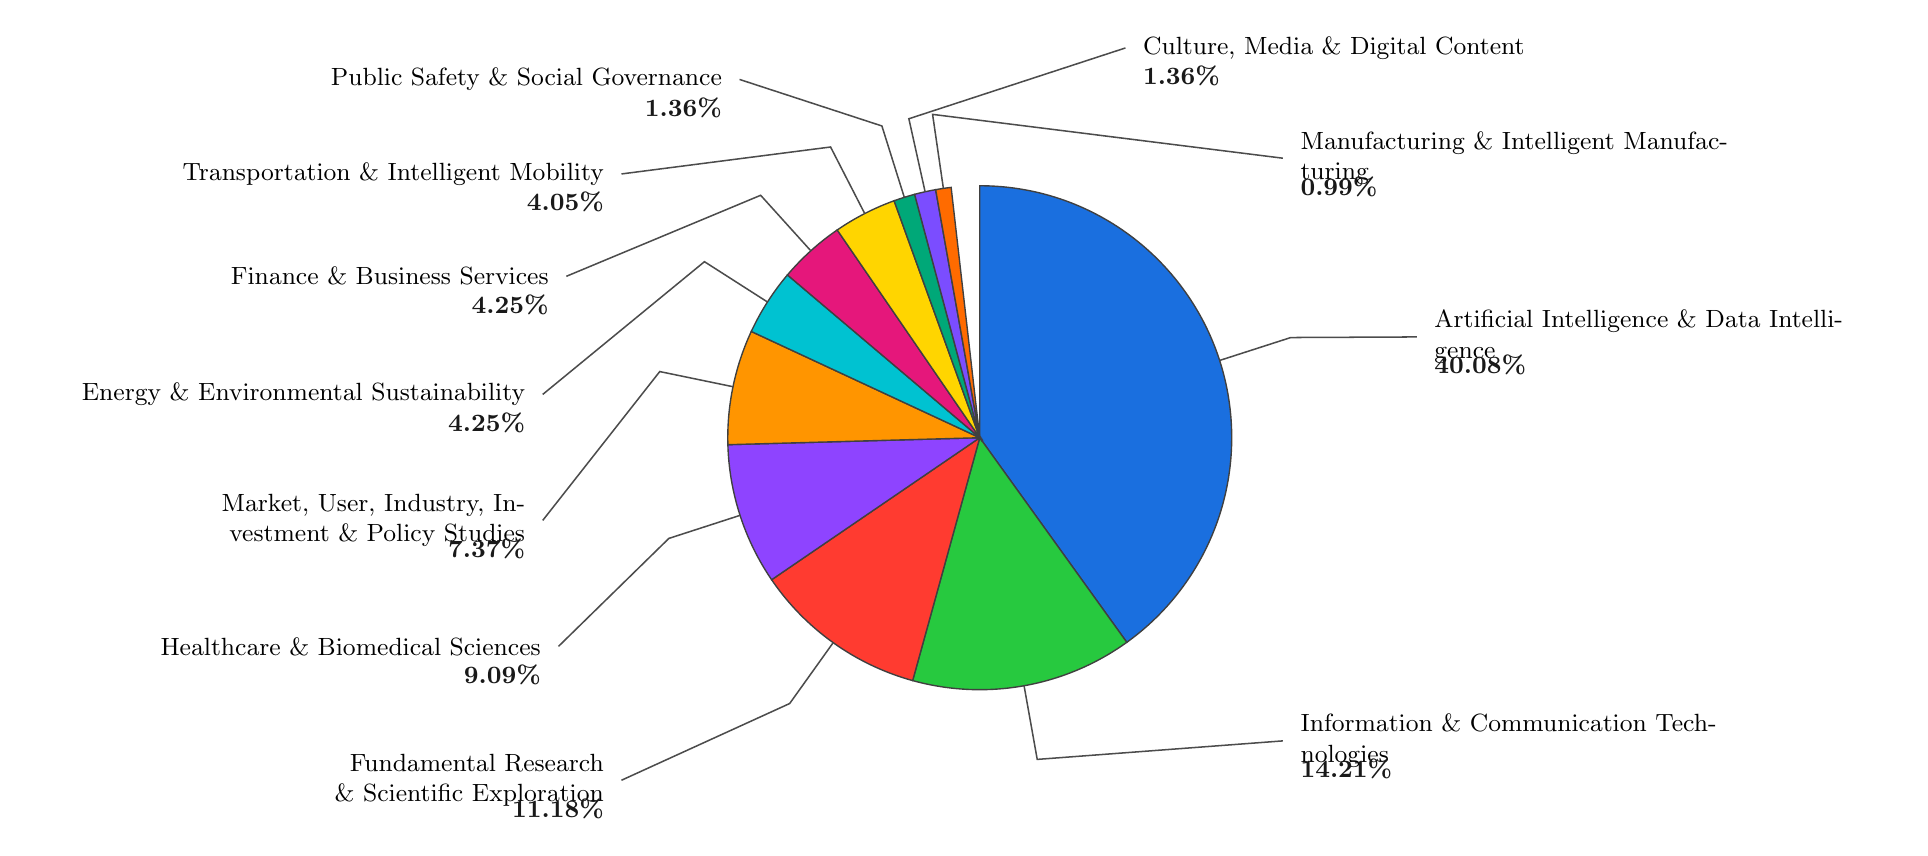
\begin{tikzpicture}[
    font=\small,
    pie/.style={
        draw=black!75,
        line width=0.5pt
    },
    labeltext/.style={
        font=\small,
        text=black,
        align=left
    },
    percenttext/.style={
        font=\small\bfseries,
        text=black!90
    },
    leader/.style={
        black!70,
        line width=0.55pt
    }
]

% ------------------------------------------------------------
% 饼图基础参数
% ------------------------------------------------------------
\def\radius{3.2}
\def\labelradius{4.15}
\def\textradius{4.55}

% ------------------------------------------------------------
% 每个扇区：起始角/结束角/中间角/颜色/百分比/标签
% 注意：角度根据百分比手动换算，整体约为 360 度
% ------------------------------------------------------------

% 40.08%
\path[pie, fill=barA]
    (0,0) -- (90:\radius)
    arc[start angle=90, end angle=-54.288, radius=\radius]
    -- cycle;
\draw[leader] (17.856:\radius) -- (17.856:\labelradius) -- (5.55,1.28);
\node[labeltext, anchor=west, text width=5.8cm] at (5.65,1.28)
    {Artificial Intelligence \& Data Intelligence};
\node[percenttext, anchor=west] at (5.65,0.92)
    {40.08\%};

% 14.21%
\path[pie, fill=barB]
    (0,0) -- (-54.288:\radius)
    arc[start angle=-54.288, end angle=-105.444, radius=\radius]
    -- cycle;
\draw[leader] (-79.866:\radius) -- (-79.866:\labelradius) -- (3.85,-3.85);
\node[labeltext, anchor=west, text width=5.6cm] at (3.95,-3.85)
    {Information \& Communication Technologies};
\node[percenttext, anchor=west] at (3.95,-4.21)
    {14.21\%};

% 11.18%
\path[pie, fill=barC]
    (0,0) -- (-105.444:\radius)
    arc[start angle=-105.444, end angle=-145.692, radius=\radius]
    -- cycle;
\draw[leader] (-125.568:\radius) -- (-125.568:\labelradius) -- (-4.55,-4.35);
\node[labeltext, anchor=east, text width=5.8cm, align=right] at (-4.65,-4.35)
    {Fundamental Research \& Scientific Exploration};
\node[percenttext, anchor=east] at (-4.65,-4.71)
    {11.18\%};

% 9.09%
\path[pie, fill=barD]
    (0,0) -- (-145.692:\radius)
    arc[start angle=-145.692, end angle=-178.416, radius=\radius]
    -- cycle;
\draw[leader] (-162.054:\radius) -- (-162.054:\labelradius) -- (-5.35,-2.65);
\node[labeltext, anchor=east, text width=5.8cm, align=right] at (-5.45,-2.65)
    {Healthcare \& Biomedical Sciences};
\node[percenttext, anchor=east] at (-5.45,-3.01)
    {9.09\%};

% 7.37%
\path[pie, fill=barE]
    (0,0) -- (-178.416:\radius)
    arc[start angle=-178.416, end angle=-204.948, radius=\radius]
    -- cycle;
\draw[leader] (-191.682:\radius) -- (-191.682:\labelradius) -- (-5.55,-1.05);
\node[labeltext, anchor=east, text width=6.2cm, align=right] at (-5.65,-1.05)
    {Market, User, Industry, Investment \& Policy Studies};
\node[percenttext, anchor=east] at (-5.65,-1.41)
    {7.37\%};

% 4.25%
\path[pie, fill=barF]
    (0,0) -- (-204.948:\radius)
    arc[start angle=-204.948, end angle=-220.248, radius=\radius]
    -- cycle;
\draw[leader] (-212.598:\radius) -- (-212.598:\labelradius) -- (-5.55,0.55);
\node[labeltext, anchor=east, text width=5.8cm, align=right] at (-5.65,0.55)
    {Energy \& Environmental Sustainability};
\node[percenttext, anchor=east] at (-5.65,0.19)
    {4.25\%};

% 4.25%
\path[pie, fill=barG]
    (0,0) -- (-220.248:\radius)
    arc[start angle=-220.248, end angle=-235.548, radius=\radius]
    -- cycle;
\draw[leader] (-227.898:\radius) -- (-227.898:\labelradius) -- (-5.25,2.05);
\node[labeltext, anchor=east, text width=5.8cm, align=right] at (-5.35,2.05)
    {Finance \& Business Services};
\node[percenttext, anchor=east] at (-5.35,1.69)
    {4.25\%};

% 4.05%
\path[pie, fill=barH]
    (0,0) -- (-235.548:\radius)
    arc[start angle=-235.548, end angle=-250.128, radius=\radius]
    -- cycle;
\draw[leader] (-242.838:\radius) -- (-242.838:\labelradius) -- (-4.55,3.35);
\node[labeltext, anchor=east, text width=5.8cm, align=right] at (-4.65,3.35)
    {Transportation \& Intelligent Mobility};
\node[percenttext, anchor=east] at (-4.65,2.99)
    {4.05\%};

% 1.36%
\path[pie, fill=barI]
    (0,0) -- (-250.128:\radius)
    arc[start angle=-250.128, end angle=-255.024, radius=\radius]
    -- cycle;
\draw[leader] (-252.576:\radius) -- (-252.576:\labelradius) -- (-3.05,4.55);
\node[labeltext, anchor=east, text width=5.8cm, align=right] at (-3.15,4.55)
    {Public Safety \& Social Governance};
\node[percenttext, anchor=east] at (-3.15,4.19)
    {1.36\%};

% 1.36%
\path[pie, fill=barJ]
    (0,0) -- (-255.024:\radius)
    arc[start angle=-255.024, end angle=-259.920, radius=\radius]
    -- cycle;
\draw[leader] (-257.472:\radius) -- (-257.472:\labelradius) -- (1.85,4.95);
\node[labeltext, anchor=west, text width=5.8cm] at (1.95,4.95)
    {Culture, Media \& Digital Content};
\node[percenttext, anchor=west] at (1.95,4.59)
    {1.36\%};

% 0.99%
\path[pie, fill=barK]
    (0,0) -- (-259.920:\radius)
    arc[start angle=-259.920, end angle=-263.484, radius=\radius]
    -- cycle;
\draw[leader] (-261.702:\radius) -- (-261.702:\labelradius) -- (3.85,3.55);
\node[labeltext, anchor=west, text width=5.8cm] at (3.95,3.55)
    {Manufacturing \& Intelligent Manufacturing};
\node[percenttext, anchor=west] at (3.95,3.19)
    {0.99\%};

\end{tikzpicture}

\end{document}
